\section{Техническое задание}
\subsection{Основание для разработки}

Основанием для разработки является задание на выпускную квалификационную работу бакалавра "<Программа аугментации изображений предназначенная для интеллектуальных систем">.

\subsection{Цель и назначение разработки}

Основной задачей выпускной квалификационной работы является разработка программы аугментации изображений предназначенная для интеллектуальных систем для компании ООО «Предприятие ВТИ-Сервис».

Программа предназначена для автоматизированной аугментации полутоновых изображений с целью генерации расширенной обучающей выборки, пригодной для последующего использования в процессе обучения нейронных сетей.

Пользовательский функционал должен обеспечивать возможность проведения аугментации даже при наличии ограниченного количества исходных изображений.

Задачами данной разработки являются:

\begin{itemize}
\item разработка модуля для аугментации полутоновых изображений с применением трансформаций;
\item реализация пользовательского интерфейса для загрузки изображений, настройки параметров аугментации и запуска отработки;
\item обеспечение поддержки пакетной обработки изображений, включая возможность работы с ограниченными выборками (менее 10 изображений);
\item реализация экспорта результатов в заданную директорию в формате PNG или JPEG;
\item валидация результатов аугментации и визуализация примеров аугментированных изображений для оценки качества преобразований.
\end{itemize}

\subsection{Требования пользователя к интерфейсу программы}

Интерфейс графического приложения должен обеспечивать:

\begin{itemize}
	\item выбор папки с изображениями для обработки;
	\item отображение количества загруженных изображений;
	\item предварительный просмотр исходного изображения;
	\item выбор уровня аугментации (low, medium, high);
	\item кнопку запуска аугментации;
	\item выбор папки для сохранения результатов;
	\item отображение предпросмотра аугментированного изображения;
	\item вывод сообщений об ошибках и успешной обработке;
	\item стильное и интуитивно понятное оформление интерфейса.
\end{itemize}

\subsubsection{Требования к данным программной системы}

Входными данными для программы являются:
\begin{itemize}
	\item папка, содержащая изображения в форматах \texttt{.jpg}, \texttt{.jpeg}, \texttt{.png}, \texttt{.bmp};
	\item выбранный пользователем уровень аугментации: \texttt{low}, \texttt{medium} или \texttt{high}.
\end{itemize}

Выходными данными для программы являются:
\begin{itemize}
	\item набор аугментированных изображений, сохранённых в указанную пользователем папку;
	\item каждое изображение имеет уникальное имя, включающее исходное имя и тип применённой аугментации (например, \texttt{image1\_rotate.jpg}), а также отформатировано в фиксированный размер.
\end{itemize}


%\begin{figure}[ht]
%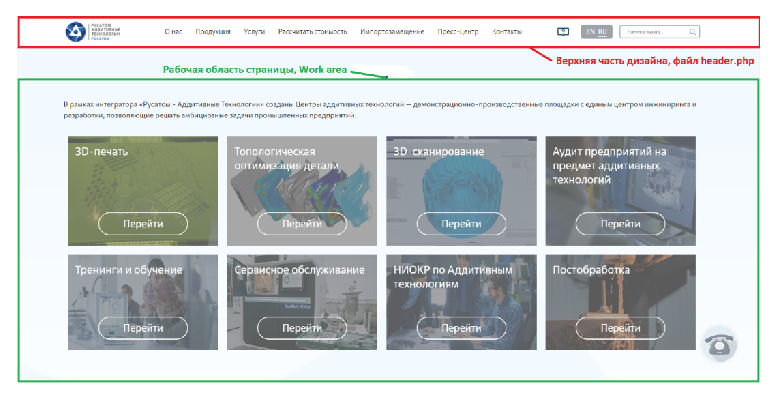
\includegraphics[width=1\linewidth]{templ}
%\caption{Композиция шаблона сайта}
%\label{templ:image}
%\end{figure}
%\vspace{-\figureaboveskip} % двойной отступ не нужен (можно использовать, если раздел заканчивается картинкой)

\subsubsection{Функциональные требования к программной системе}

Разрабатываемая система должна обеспечивать следующие функции:

\begin{itemize}
	\item загрузка изображений из выбранной пользователем папки;
	\item отображение количества загруженных изображений;
	\item отображение предварительного просмотра одного из загруженных изображений;
	\item выбор уровня аугментации: низкий (low), средний (medium), высокий (high);
	\item выбор папки для сохранения аугментированных изображений;
	\item применение набора аугментаций к каждому изображению с учётом выбранного уровня;
	\item сохранение результатов в заданную папку с указанием типа аугментации в названии файлов;
	\item предпросмотр одного из аугментированных изображений после завершения обработки;
	\item отображение сообщений об ошибках при отсутствии изображений, путей или некорректных действиях.
\end{itemize}

На рисунке 2.1 в виде диаграммы прецедентов [10] представлены функциональные требования к системе, доступные для обеих категорий пользователей.

\begin{figure}[H]
	\centering
	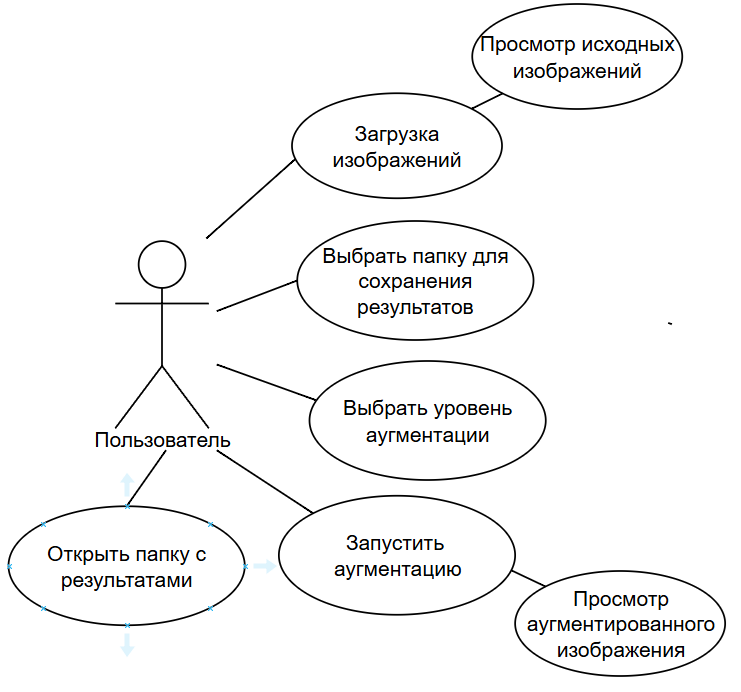
\includegraphics[width=0.7\linewidth]{images/diagrampreced}
	\caption{Диаграмма прецедентов}
	\label{fig:diagrampreced}
\end{figure}


\paragraph{Вариант использования «Загрузка изображений»}

Заинтересованные лица и их требования:
Пользователь желает загрузить изображения из локальной папки для дальнейшей обработки.
Предусловие:
Программа запущена, главное окно отображается.
Постусловие:
Список изображений успешно загружен и готов к обработке. Отображается предварительный просмотр одного изображения.
Основной успешный сценарий:
\begin{enumerate}
	\item Пользователь нажимает кнопку «Загрузить папку».
	\item Открывается стандартный диалог выбора папки.
	\item Пользователь выбирает папку, содержащую изображения.
	\item Программа считывает все подходящие файлы по расширениям (.jpg, .jpeg, .png, .bmp).
	\item Если изображения найдены — отображается их количество и предварительный просмотр одного изображения.
	\item Если изображения отсутствуют — отображается предупреждение.
\end{enumerate}

\paragraph{Вариант использования «Выбор папки для сохранения»}

Заинтересованные лица и их требования:
Пользователь хочет указать папку, куда будут сохранены результаты аугментации.
Предусловие:
Программа запущена. Загружены изображения.
Постусловие:
Путь для сохранения результатов успешно сохранён и отображается в интерфейсе.
Основной успешный сценарий:

\begin{enumerate}
	\item Пользователь нажимает кнопку «Выбрать папку для сохранения».
	\item Открывается стандартный диалог выбора папки.
	\item Пользователь выбирает папку.
	\item Путь к папке отображается в информационном блоке программы.
\end{enumerate}

\paragraph{Вариант использования «Выбор уровня аугментации»}

Заинтересованные лица и их требования:
Пользователь хочет определить интенсивность применяемых преобразований к изображениям.
Предусловие:
Программа запущена, изображения загружены.
Постусловие:
Уровень аугментации (low, medium, high) выбран и сохранён до момента применения обработки.
Основной успешный сценарий:

\begin{enumerate}
	\item Пользователь нажимает на выпадающий список.
	\item Пользователь выбирает один из доступных уровней.
	\item Программа сохраняет выбранный уровень для дальнейшей обработки.
\end{enumerate}

\paragraph{Вариант использования «Применение аугментации»}

Заинтересованные лица и их требования:
Пользователь хочет обработать загруженные изображения с применением выбранных методов.
Предусловие:
Загружены изображения, выбран уровень аугментации и папка для сохранения.
Постусловие:
Аугментированные изображения сохранены в выбранную папку. Отображается сообщение об успешном завершении.
Основной успешный сценарий:

\begin{enumerate}
	\item Пользователь нажимает кнопку «Применить аугментацию».
	\item Программа проверяет, загружены ли изображения и выбрана ли папка.
	\item Каждое изображение предварительно масштабируется и передаётся в модуль обработки.
	\item Модуль обработки применяет выбранные аугментации.
	\item Результаты сохраняются с модифицированными именами в выбранной папке.
	\item Программа отображает сообщение об успешной обработке.
\end{enumerate}

\paragraph{Вариант использования «Предпросмотр изображений»}

Заинтересованные лица и их требования:
Пользователь хочет увидеть исходное изображение и результат аугментации для визуальной оценки.
Предусловие:
Изображения загружены, аугментация завершена.
Постусловие:
В интерфейсе отображается пара: оригинал и результат аугментации.
Основной успешный сценарий:

\begin{enumerate}
	\item После завершения аугментации, программа отображает исходное изображение и один из полученных результатов.
	\item Пользователь визуально оценивает результат на встроенных миниатюрах (QLabel).
\end{enumerate}

\paragraph{Вариант использования «Предпросмотр изображений до и после»}

Заинтересованные лица и их требования:
Пользователь хочет визуально сравнить исходное изображение и результат аугментации.
Предусловие:
Минимум одно изображение успешно обработано. В интерфейсе доступна панель предпросмотра.
Постусловие:
На экране отображаются миниатюры: исходное и аугментированное изображение. Пользователь может переходить к следующей паре.
Основной успешный сценарий:

\begin{enumerate}
	\item После завершения аугментации, интерфейс отображает первое изображение до обработки и один из его аугментированных вариантов.
	\item Под предпросмотром расположены кнопки: «Предыдущее», «Следующее».
	\item При нажатии на «Следующее», отображается следующая пара (оригинал и результат).
	\item Если достигнут конец списка, кнопка «Следующее» становится недоступной.
	\item Аналогично работает кнопка «Предыдущее».
\end{enumerate}

\paragraph{Вариант использования «Открытие папки с аугментированными изображениями»}

Заинтересованные лица и их требования:
Пользователь хочет быстро открыть в проводнике папку с готовыми результатами.
Предусловие:
Папка для сохранения результатов была выбрана, аугментация успешно завершена.
Постусловие:
Открывается системный файловый менеджер в выбранной ранее директории.
Основной успешный сценарий:
\begin{enumerate}
	\item Пользователь нажимает кнопку «Открыть папку с результатами».
	\item Программа проверяет наличие валидного пути к папке.
	\item Если путь существует, открывается стандартный проводник (используется QDesktopServices.openUrl()).
	\item Если путь не был указан или папка недоступна, появляется сообщение об ошибке.
\end{enumerate}

\subsection{Вариант использования «Загрузка изображений»}

Разработка программной документации и программного изделия должна производиться согласно ГОСТ 19.102-77 и ГОСТ 34.601-90. Единая система программной документации.

Программная документация должна включать в себя:
\begin{itemize}
	\item анализ предметной области;
	\item техническое задание;
	\item технический проект;
	\item рабочий проект.
\end{itemize}
